% The defense presentation of the thesis. Figures, model names and references come from
% ../monografia; third-party material lives in third_party/, which is not versioned.
% Build: latexmk -pdf presentation.tex. Present: pdfpc presentation.pdf.
\documentclass[aspectratio=169]{beamer}

\usepackage[utf8]{inputenc}
\usepackage[T1]{fontenc}
\usepackage[english]{babel}
\usepackage{amsmath,amssymb}
\usepackage{booktabs}
\usepackage{listings}
\usepackage{xspace}
\usepackage{seqsplit}
\usepackage{abntex2abrev}
\usepackage{cite}
\usepackage{qrcode}
\usepackage{appendixnumberbeamer}
\usepackage[overridenote]{pdfpc}
\pdfpcsetup{duration=20, lastminutes=3}

\newcommand{\modelname}[1]{\textbf{#1}\xspace}
\newcommand{\datasetname}[1]{\textbf{#1}\xspace}
\newcommand{\variant}[1]{\textit{#1}\xspace}
\newcommand{\codename}[1]{\texttt{\protect\seqsplit{#1}}}
\newcommand{\MicroTEDAClus}{\modelname{MicroTEDAClus}}
\newcommand{\MicroTEDAClusPlus}{\modelname{MicroTEDAClus+}}
\newcommand{\StreamKM}{\modelname{StreamKM}}
\newcommand{\DenStream}{\modelname{DenStream}}
\newcommand{\CluStream}{\modelname{CluStream}}
\newcommand{\CEDAS}{\modelname{CEDAS}}
\newcommand{\TEDACloud}{\modelname{TEDACloud}}
\newcommand{\AutoCloud}{\modelname{AutoCloud}}
\newcommand{\Cassini}{\datasetname{Cassini}}
\newcommand{\BenchmarkOne}{\datasetname{StreamBenchmark(1)}}
\newcommand{\BenchmarkTwo}{\datasetname{StreamBenchmark(2)}}
\newcommand{\RandomRBFGeneratorEvents}{\datasetname{RandomRBFGeneratorEvents}}
\newcommand{\ChameleonDSThree}{\datasetname{DS3}}
\newcommand{\ChameleonDSFour}{\datasetname{DS4}}
\newcommand{\DBSTREAM}{\modelname{DBSTREAM}}
\newcommand{\BIRCH}{\modelname{BIRCH}}
\newcommand{\MiniBatchKMeans}{\modelname{Mini-batch k-means}}
\newcommand{\BICO}{\modelname{BICO}}
\newcommand{\InsectsAbrupt}{\datasetname{INSECTS abrupt}}
\newcommand{\InsectsIncremental}{\datasetname{INSECTS incremental}}
\newcommand{\InsectsReoccurring}{\datasetname{INSECTS incremental-reoccurring}}
\newcommand{\GasDrift}{\datasetname{Gas Sensor Array Drift}}
\newcommand{\KDDCup}{\datasetname{KDD Cup 1999}}
\newcommand{\Covertype}{\datasetname{Forest Covertype}}
\newcommand{\Pendigits}{\datasetname{Pendigits}}
\newcommand{\Shuttle}{\datasetname{Shuttle}}

\graphicspath{{../monografia/}}

\setbeamertemplate{navigation symbols}{}
\setbeamertemplate{footline}[frame number]
\setbeamertemplate{bibliography item}[text]

\lstset{%
  basicstyle=\ttfamily\scriptsize,
  columns=fullflexible,
  frame=single,
  keepspaces=true,
  tabsize=4,
  keywordstyle=\color{blue},
  commentstyle=\color{gray},
  stringstyle=\color{green!50!black},
}

% A grey box that stands for content still to be made.
\newcommand{\placeholder}[3]{%
  \fcolorbox{gray}{gray!10}{\parbox[c][#2][c]{\dimexpr#1-2\fboxsep-2\fboxrule\relax}{\centering\footnotesize\color{gray!70!black}#3}}}
% A file if it exists, otherwise a placeholder of the same size.
\newcommand{\maybegraphics}[4]{%
  \IfFileExists{#3}{\includegraphics[width=#1,height=#2,keepaspectratio]{#3}}{\placeholder{#1}{#2}{#4}}}
% The terms of an equation that the slide points at.
\newcommand{\hl}[1]{{\color{red!75!black}#1}}

\title{MicroTEDAClus Formulation, Implementation, and Experimental Validation Reassessment and Improvement}
\author{Eduardo Henrique Basilio de Carvalho}
\institute{Advisor: Prof.\ Janier Arias Garcia, PhD\\[2pt]
  Bachelor's Degree in Control and Automation Engineering\\Federal University of Minas Gerais}
\date{November 23, 2026}

\begin{document}

\begin{frame}
  \titlepage
  \note{- Greet the board\\- Title: reassessment and improvement of MicroTEDAClus}
\end{frame}

% -----------------------------------------------------------------------------
\section{The online stream clustering problem}

\begin{frame}{Clustering a data stream}
  \begin{columns}[c]
    \column{0.45\textwidth}
    \begin{itemize}
      \item Samples arrive without a known end
      \item Each batch: predict its labels, then learn it
      \item A bounded summary instead of the data
      \item The process may change: concept drift
    \end{itemize}
    \column{0.5\textwidth}
    \placeholder{\linewidth}{0.6\textheight}{Batches of a stream with concept drift\\(slide figure to make from the datasets)}
  \end{columns}
  \note{- Superficial: the board knows it\\- Stress predict-then-learn: it returns in the critiques}
\end{frame}

\begin{frame}{Microclusters, macroclusters and the ARI}
  \begin{columns}[c]
    \column{0.5\textwidth}
    \begin{itemize}
      \item Microclusters summarize regions of the stream
      \item Macroclusters join intersecting microclusters: the clusters
      \item Quality of a batch: the adjusted Rand index
    \end{itemize}
    \[
      \mathrm{ARI} = \frac{\mathrm{RI} - \mathbb{E}[\mathrm{RI}]}{\max \mathrm{RI} - \mathbb{E}[\mathrm{RI}]}
    \]
    \begin{itemize}
      \item 1: perfect agreement; about 0: chance
    \end{itemize}
    \column{0.45\textwidth}
    \placeholder{\linewidth}{0.6\textheight}{Microclusters and their macroclusters\\(diagram to make)}
  \end{columns}
  \note{- One sentence each\\- Every result later is an ARI}
\end{frame}

% -----------------------------------------------------------------------------
\section{Motivation}

\begin{frame}{MicroTEDAClus and the works built on it}
  \begin{columns}[t]
    \column{0.32\textwidth}
    \centering
    \maybegraphics{\linewidth}{0.38\textheight}{third_party/maia2020.png}{Title of Maia et al.\\(your screenshot)}\\[4pt]
    \footnotesize Maia et al.~\cite{maia2020evolvclus}\\
    on par with established algorithms; adapts better to concept drift
    \column{0.32\textwidth}
    \centering
    \maybegraphics{\linewidth}{0.38\textheight}{third_party/galindo2021.png}{Title of Galindo\\(your screenshot)}\\[4pt]
    \footnotesize Galindo~\cite{galindo2021lastmile}\\
    updates the algorithm; applies it to last-mile logistics
    \column{0.32\textwidth}
    \centering
    \maybegraphics{\linewidth}{0.38\textheight}{third_party/cardoso2022.png}{Title of Cardoso\\(your screenshot)}\\[4pt]
    \footnotesize Cardoso~\cite{cardoso2022microtedaclus}\\
    reimplements it in C; expects it to handle drift
  \end{columns}
  \note{- The published results are the basis of later work\\- A model whose evaluation supports further work must be verified}
\end{frame}

\begin{frame}{Objectives}
  \begin{enumerate}[a)]
    \item Examine the formulation of \MicroTEDAClus and its public implementation
    \item Examine the methodology of the original experiments, and define one without its flaws
    \item Evaluate \MicroTEDAClus against benchmark models under that methodology
    \item Propose an improved model, and evaluate it under the same methodology
  \end{enumerate}
  \note{- Objectives a and b: the critiques\\- Objective c: Chapter 3\\- Objective d: Chapter 4}
\end{frame}

% -----------------------------------------------------------------------------
\section{The formulation and its implementation}

\begin{frame}{A dimensionality penalty}
  TEDA, as Maia et al.\ write it~\cite{angelov2014outside,maia2020evolvclus}:
  \[
    \xi(x_k) = \frac{1}{k} + \frac{(\mu_k - x_k)^T(\mu_k - x_k)}{k\,\sigma^2_k}
  \]
  \MicroTEDAClus, for a microcluster $i$ with $S^i_k$ samples:
  \begin{gather*}
    (\sigma^i_k)^2 = \frac{S^i_k - 1}{S^i_k}(\sigma^i_{k-1})^2 + \frac{1}{S^i_k - 1}\left(\frac{2\lVert x_k - \mu^i_k\rVert}{\hl{d}}\right)^2\\
    \xi^i(x_k) = \frac{1}{S^i_k} + \frac{2(\mu^i_k - x_k)^T(\mu^i_k - x_k)}{S^i_k(\sigma^i_k)^2\,\hl{d}}
  \end{gather*}
  \begin{itemize}
    \item No paper of the TEDA metrics scales by the dimension $d$, and the original work does not justify it
    \item The normalized eccentricity can exceed its bound of one half
    \item Its consequence: the collapse in high dimensions, later
  \end{itemize}
  \note{- Point at the two d\\- Forward reference: the 64-dimension collapse}
\end{frame}

\begin{frame}[fragile]{An unreported decay}
\begin{lstlisting}[language=Python]
def prune_micro_clusters(self):
    for mc in self.micro_clusters:
        if not mc["active"]:
            mc["life"] = mc["life"] - self.fading_factor
            if mc["life"] < 0:
                self.micro_clusters.remove(mc)
\end{lstlisting}
\begin{lstlisting}[language=Python]
def update_life(self, xk, micro_cluster):
    ...
    micro_cluster["life"] = micro_cluster["life"] + (((rt - dist) / rt) * self.fading_factor)
\end{lstlisting}
  \begin{itemize}
    \item The hyperparameter \texttt{decay} becomes \texttt{fading\_factor} $= 1/\text{decay}$
    \item The paper reports no decay; the code that produced its results prunes microclusters
    \item The same rate $\rho = 1/\text{decay}$ appears later in Galindo~\cite{galindo2021lastmile}
  \end{itemize}
  \note{- The implementation, not the paper, produced the results\\- Other departures: appendix}
\end{frame}

% -----------------------------------------------------------------------------
\section{The methodology of the original experiments}

\begin{frame}{Preprocessing that leaks}
  \centering
  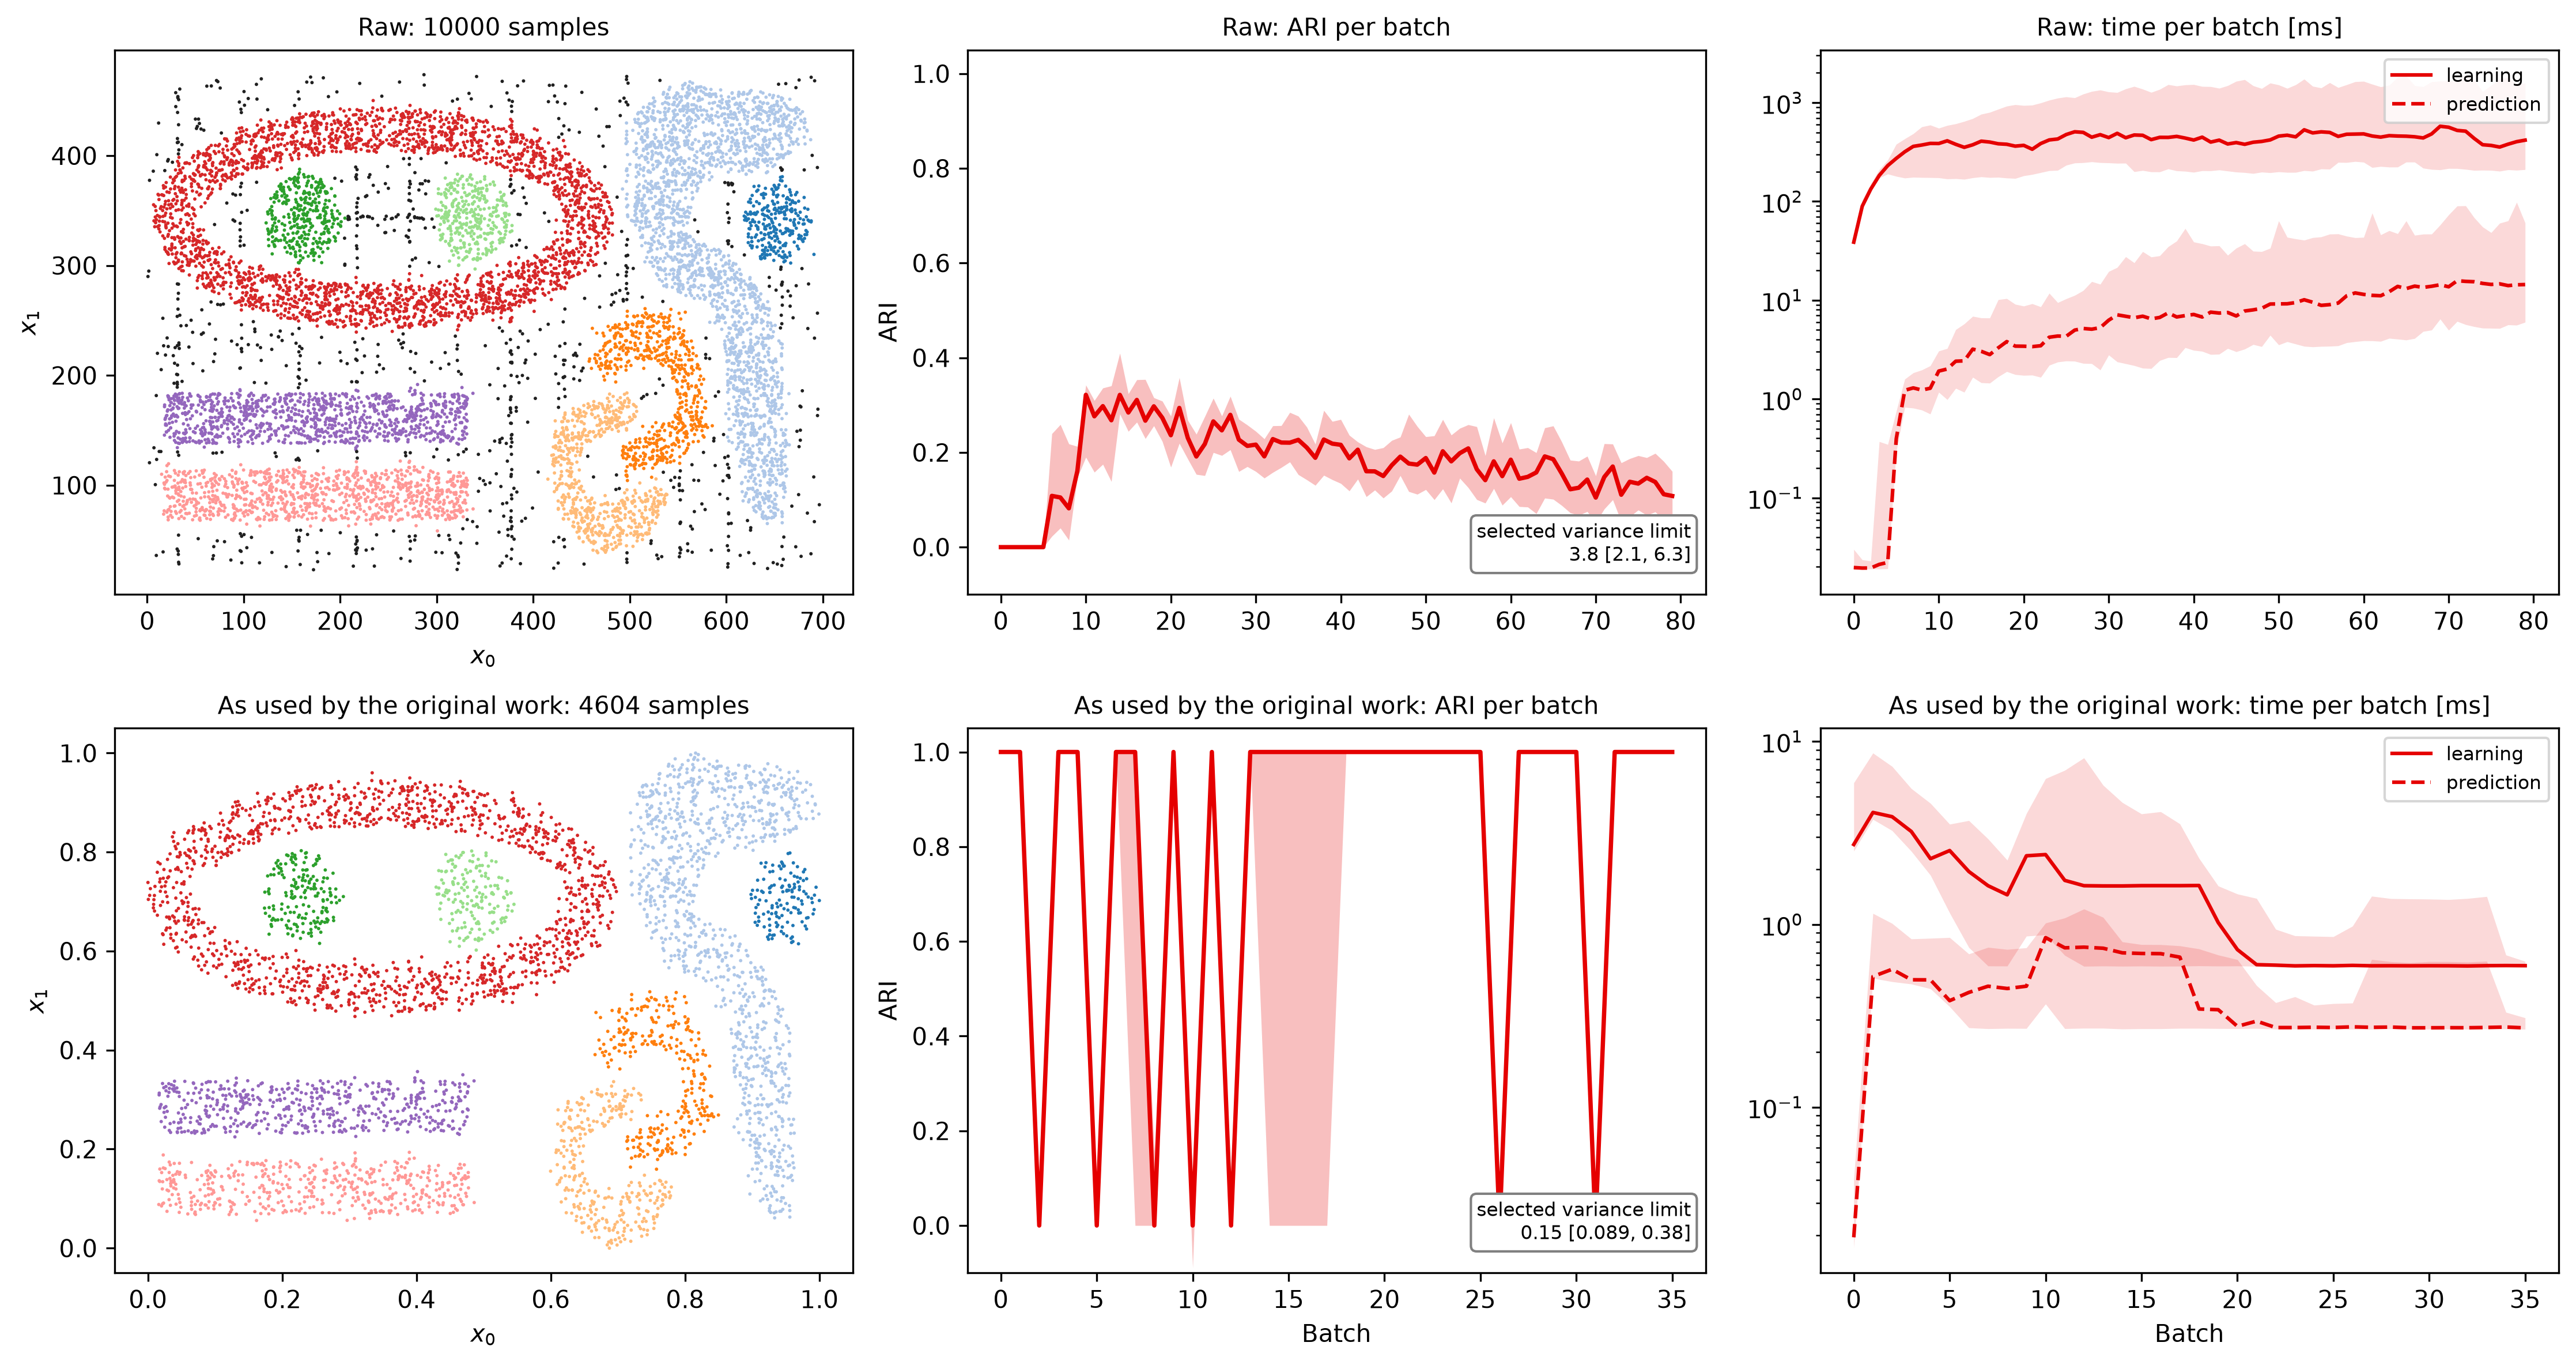
\includegraphics[height=0.62\textheight]{MethodologyReassessment/artifacts/preprocessing/ds3.png}
  \vfill
  \footnotesize
  \begin{columns}[t]
    \column{0.3\textwidth}\centering Noise removed:\\needs the labels
    \column{0.3\textwidth}\centering Min--max scaling over the stream:\\uses the future
    \column{0.3\textwidth}\centering Ordered by label:\\one cluster per batch
  \end{columns}
  \note{- Top: raw DS3; bottom: as the original work used it\\- ARI one in most batches, faster, a smaller variance limit\\- Downsampling alone does not leak}
\end{frame}

\begin{frame}[fragile]{Learn, then predict}
  \begin{columns}[c]
    \column{0.44\textwidth}
    The original evaluation of the static datasets:
\begin{lstlisting}[language=Python]
evol_model.fit(X)
y_hat = evol_model.predict(X)
error = adjusted_rand_score(y, y_hat)
\end{lstlisting}
    \placeholder{\linewidth}{0.3\textheight}{Timeline: predict then learn,\\against learn then predict\\(diagram to make)}
    \column{0.54\textwidth}
    \centering
    \maybegraphics{\linewidth}{0.6\textheight}{third_party/original_curves.png}{Published curves of Maia et al.}\\
    \footnotesize Published curves~\cite{maia2020evolvclus}: the first batch exceeds 0.5 in every one
  \end{columns}
  \note{- Stated as prequential, executed learn-then-predict\\- Prequential: the first batch is predicted before anything is learned, near zero}
\end{frame}

% -----------------------------------------------------------------------------
\section{The later works}

\begin{frame}{What the later works inherit}
  \centering
  \begin{tabular}{lp{0.18\textwidth}p{0.24\textwidth}p{0.3\textwidth}}
    \toprule
    & Dimensionality penalty & Decay & Evaluation \\
    \midrule
    Galindo~\cite{galindo2021lastmile} & kept & made explicit, $\rho = 1/\text{decay}$ & not examined \\
    Cardoso~\cite{cardoso2022microtedaclus} & \hl{to verify} & \hl{to verify} & learns each static dataset before labeling it \\
    \bottomrule
  \end{tabular}
  \note{- Both build on results whose evaluation is flawed\\- Cardoso: best grid configurations, no benchmark, no drift}
\end{frame}

% -----------------------------------------------------------------------------
\section{Our protocol}

\begin{frame}{The protocol of the reassessment}
  \begin{columns}[t]
    \column{0.5\textwidth}
    \begin{itemize}
      \item Raw streams, no preprocessing
      \item Prequential: predict each batch, then learn it
      \item First 20\%: tuning, the same budget for every model
      \item Remaining 80\%: evaluation, never seen by the search
      \item 94 runs, medians and interquartile ranges
    \end{itemize}
    \column{0.46\textwidth}
    \[
      \text{Overall ARI} = \operatorname*{median}_{b \,\in\, \text{evaluation}} \mathrm{ARI}_b
    \]
    \[
      \text{Steady-State ARI} = \mathrm{ARI}_{B-1}
    \]
    Better when, over the runs, both hold:
    \[
      p_{\text{Holm}} < 0.05, \ \text{paired Wilcoxon}
    \]
    \[
      |\delta| \ge 0.147, \ \text{Cliff's delta}
    \]
  \end{columns}
  \note{- Penultimate batch: after any drift, the last may be incomplete\\- 94 runs: the knee of the convergence curve, appendix\\- Cliff's delta: a small effect at least}
\end{frame}

% -----------------------------------------------------------------------------
\section{MicroTEDAClus under the protocol}

\begin{frame}{\MicroTEDAClus under the protocol}
  \begin{columns}[c]
    \column{0.42\textwidth}
    \begin{itemize}
      \item Not on par with the benchmark models
      \item Does not adapt better to concept drift
      \item Learns slowly
      \item Its quality collapses in high dimensions
      \item Its variance limit depends on the scale
    \end{itemize}
    \column{0.54\textwidth}
    \placeholder{\linewidth}{0.62\textheight}{Verdicts of \MicroTEDAClus against each benchmark model,\\per dataset and metric\\(figure to make)}
  \end{columns}
  \note{- The claims of the original work do not hold}
\end{frame}

\begin{frame}{The collapse in high dimensions}
  \centering
  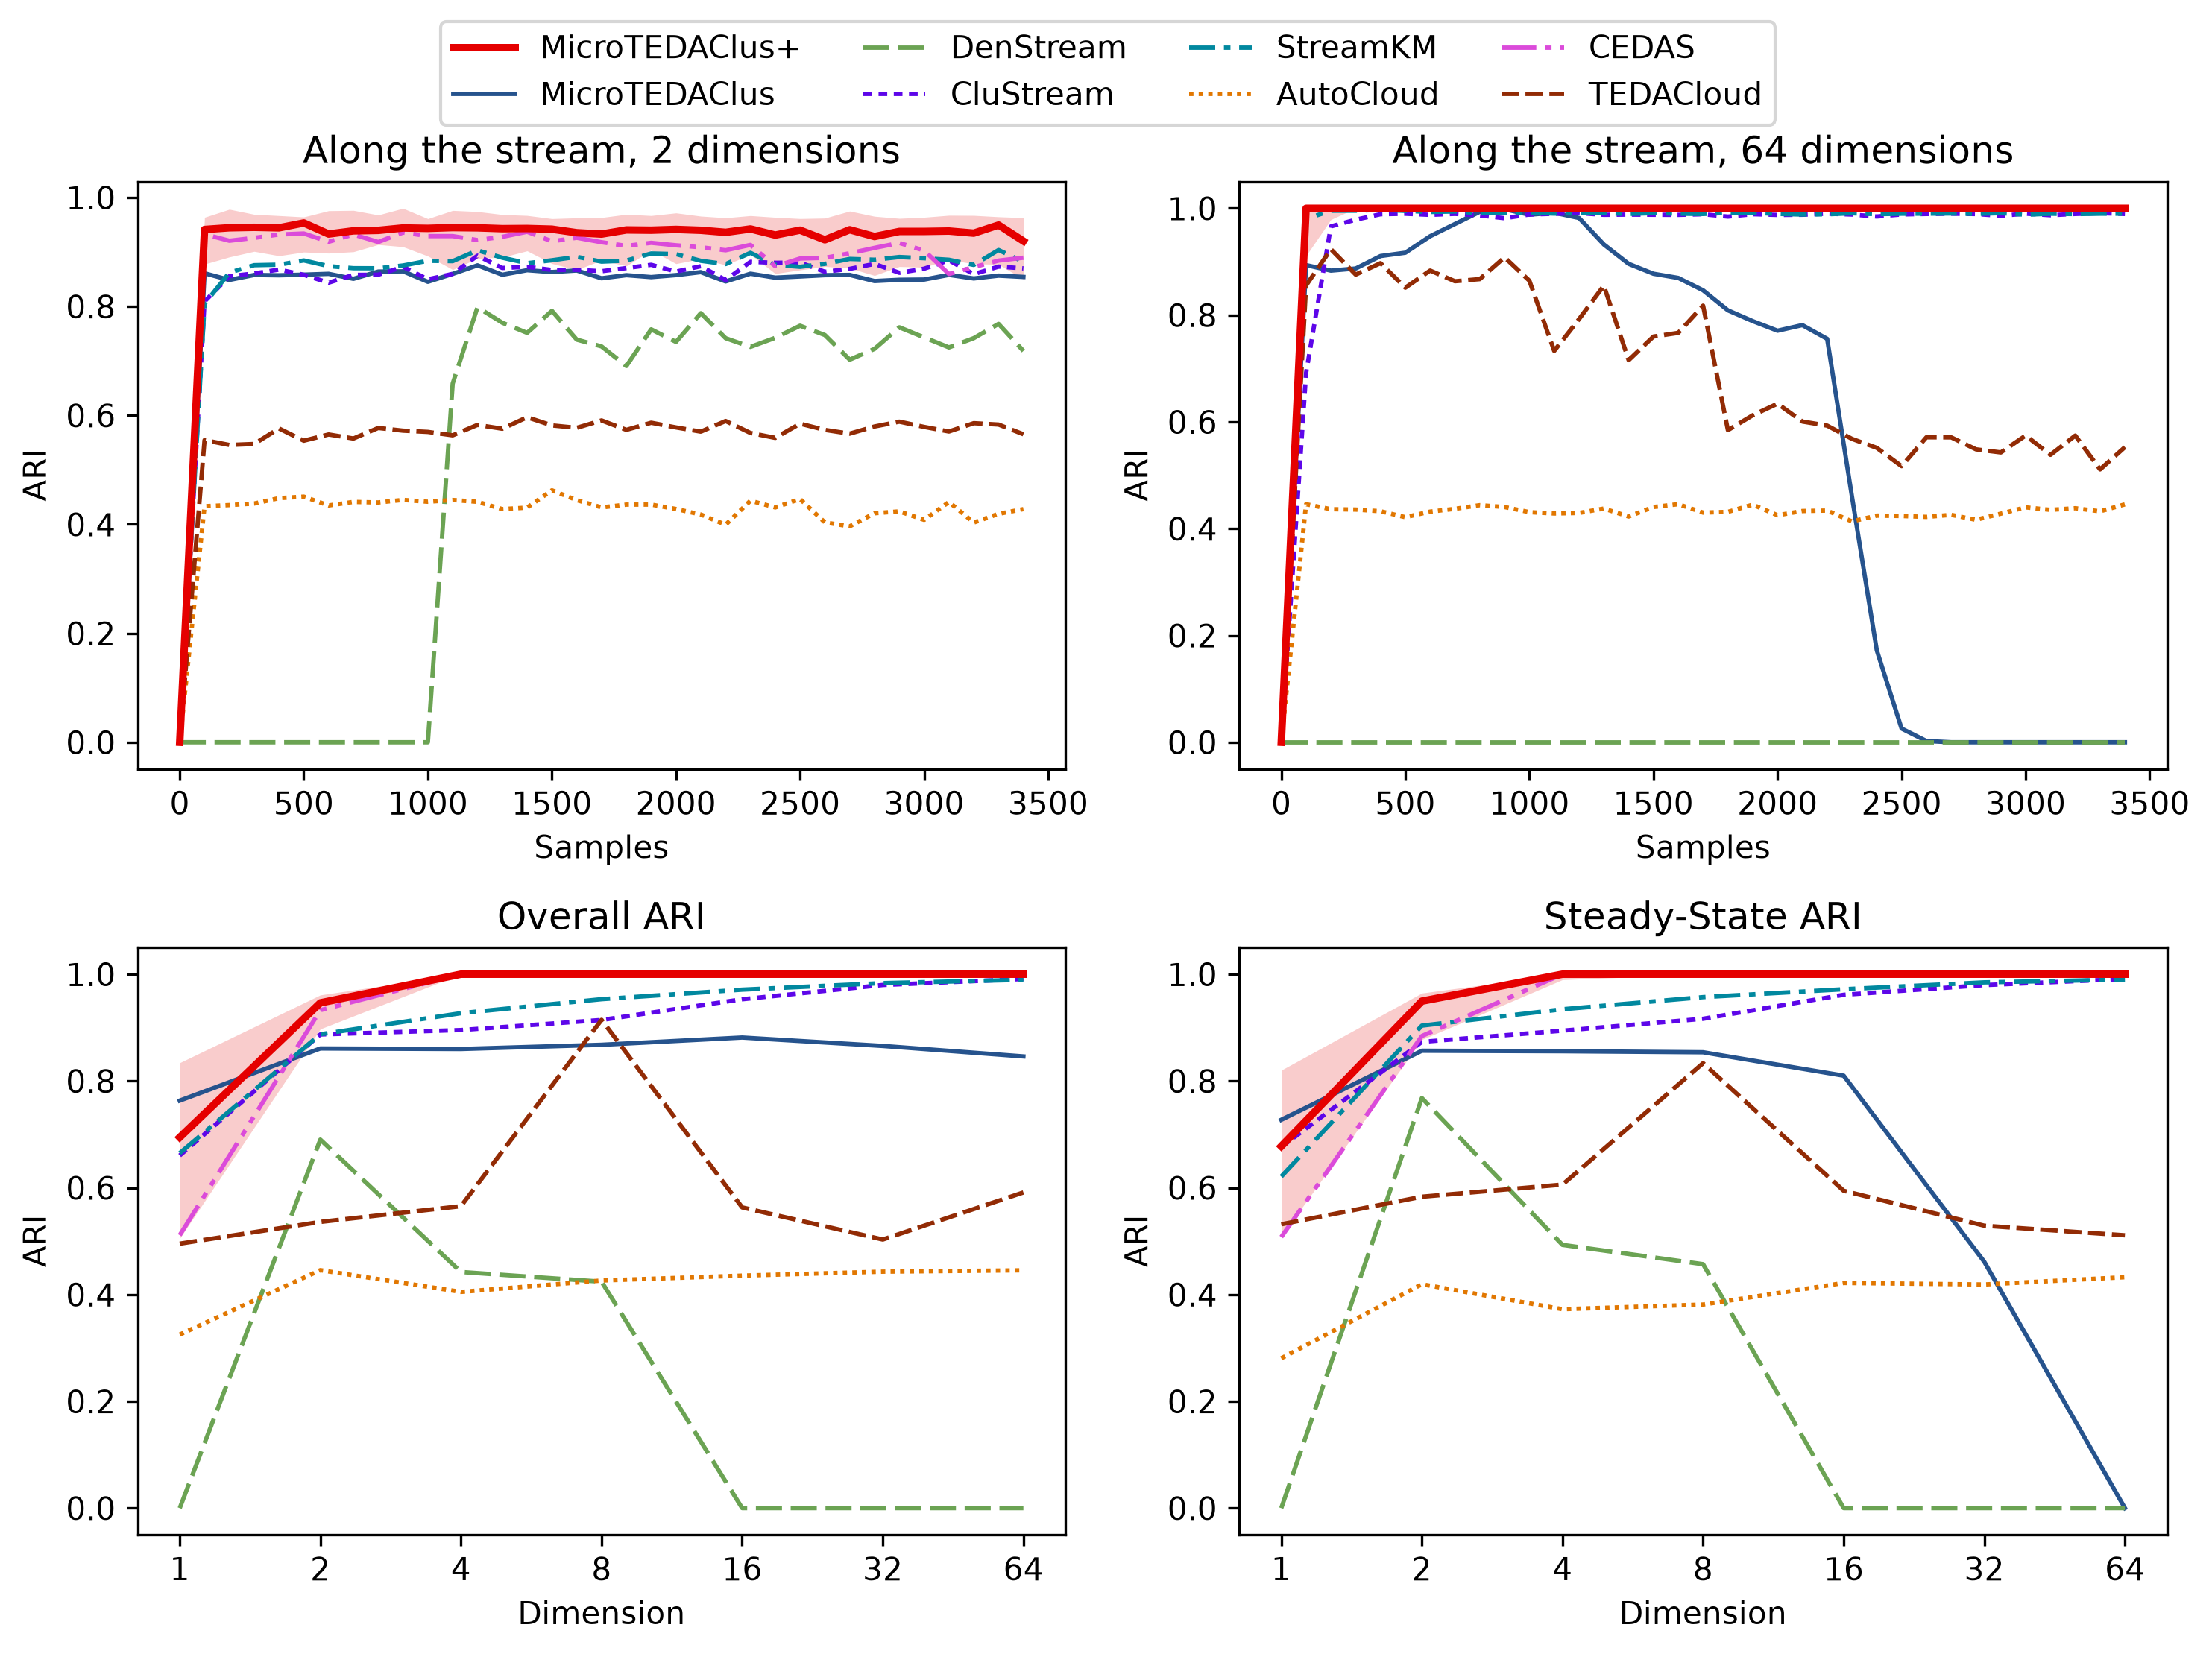
\includegraphics[height=0.8\textheight]{ModelImprovement/artifacts/comparison/plots/scalability_quality.png}
  \note{- Blue: MicroTEDAClus falls to zero with 64 dimensions\\- Replace with the version without MicroTEDAClus+}
\end{frame}

% -----------------------------------------------------------------------------
\section{From MicroTEDAClus to MicroTEDAClus+}

\begin{frame}{Five differences}
  \centering
  \small
  \begin{tabular}{p{0.15\textwidth}p{0.36\textwidth}p{0.36\textwidth}}
    \toprule
    & \MicroTEDAClus & \MicroTEDAClusPlus \\
    \midrule
    Membership & macrocluster with the largest density-weighted sum of $1 - \zeta$ & macrocluster of the active microcluster with the smallest standardized distance \\
    Update & every microcluster that accepts the sample & the nearest microcluster that accepts the sample \\
    Noise & every sample is assigned to a macrocluster & farther than $n_\sigma$ standard deviations from every active microcluster \\
    Variance limit & absolute, $r_0$ & relative to the stream, $r_0 = r\,\sigma^2_{\text{stream}}$ \\
    Distances & scaled by $2/d$ & not scaled \\
    \bottomrule
  \end{tabular}
  \note{- One correction: nearest membership\\- Three improvements: single assignment, noise label, relative limit\\- One refinement: no penalty}
\end{frame}

\begin{frame}{The chain of changes}
  \centering
  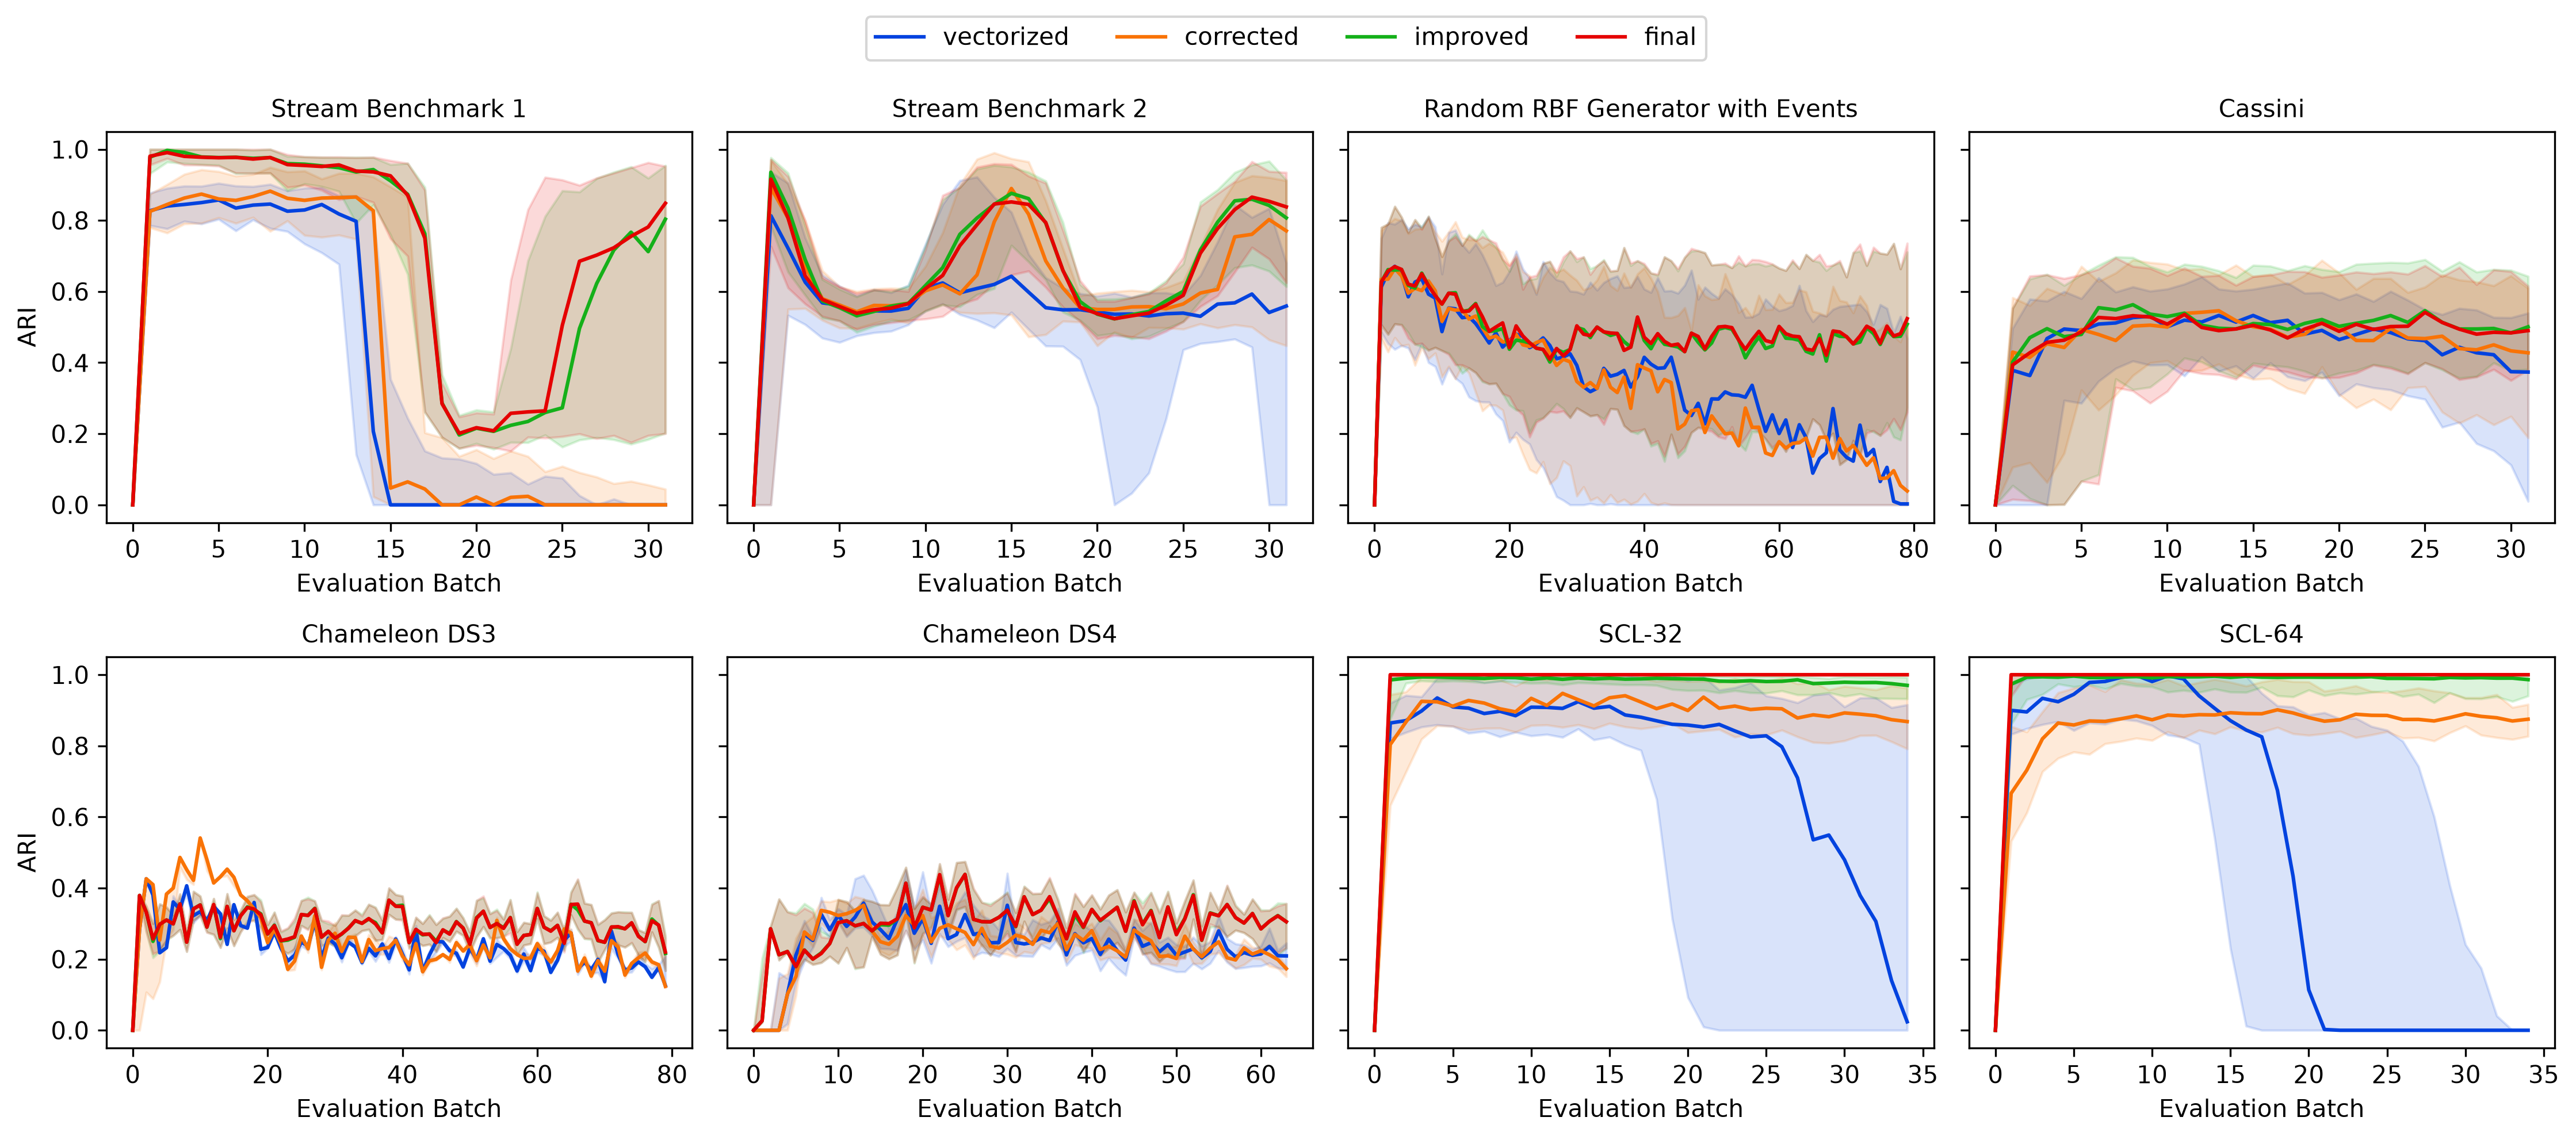
\includegraphics[width=\textwidth]{ModelImprovement/artifacts/validation/plots/ari_trajectories.png}\\[2pt]
  \footnotesize Not retained: the density reformulations, the reparameterizations of the function $m$
  \note{- Validation runs, never used in the development\\- Each step accepted by the decision rule}
\end{frame}

\begin{frame}{A vectorized implementation}
  \centering
  \placeholder{0.8\textwidth}{0.7\textheight}{Speedup of the vectorized implementation over the original one\\(figure to regenerate with the thesis palette)}
  \note{- Same results, a fraction of the time}
\end{frame}

% -----------------------------------------------------------------------------
\section{MicroTEDAClus+ under the protocol}

\begin{frame}{\MicroTEDAClusPlus under the protocol}
  \begin{columns}[c]
    \column{0.42\textwidth}
    \small
    \begin{itemize}
      \item Better than \MicroTEDAClus: Overall ARI in five of six datasets, Steady-State ARI in all six
      \item No benchmark model is better in the streams with concept drift
      \item No collapse in high dimensions
      \item The fastest model in both stages
      \item Its variance limit no longer depends on the scale
      \item Weakness: static shapes, where \CluStream and \StreamKM remain better
    \end{itemize}
    \column{0.54\textwidth}
    \placeholder{\linewidth}{0.62\textheight}{Verdicts of \MicroTEDAClusPlus against \MicroTEDAClus and each benchmark model\\(figure to make)}
  \end{columns}
  \note{- Memory: smaller than MicroTEDAClus and CluStream, larger than CEDAS and TEDACloud}
\end{frame}

\begin{frame}{In high dimensions}
  \centering
  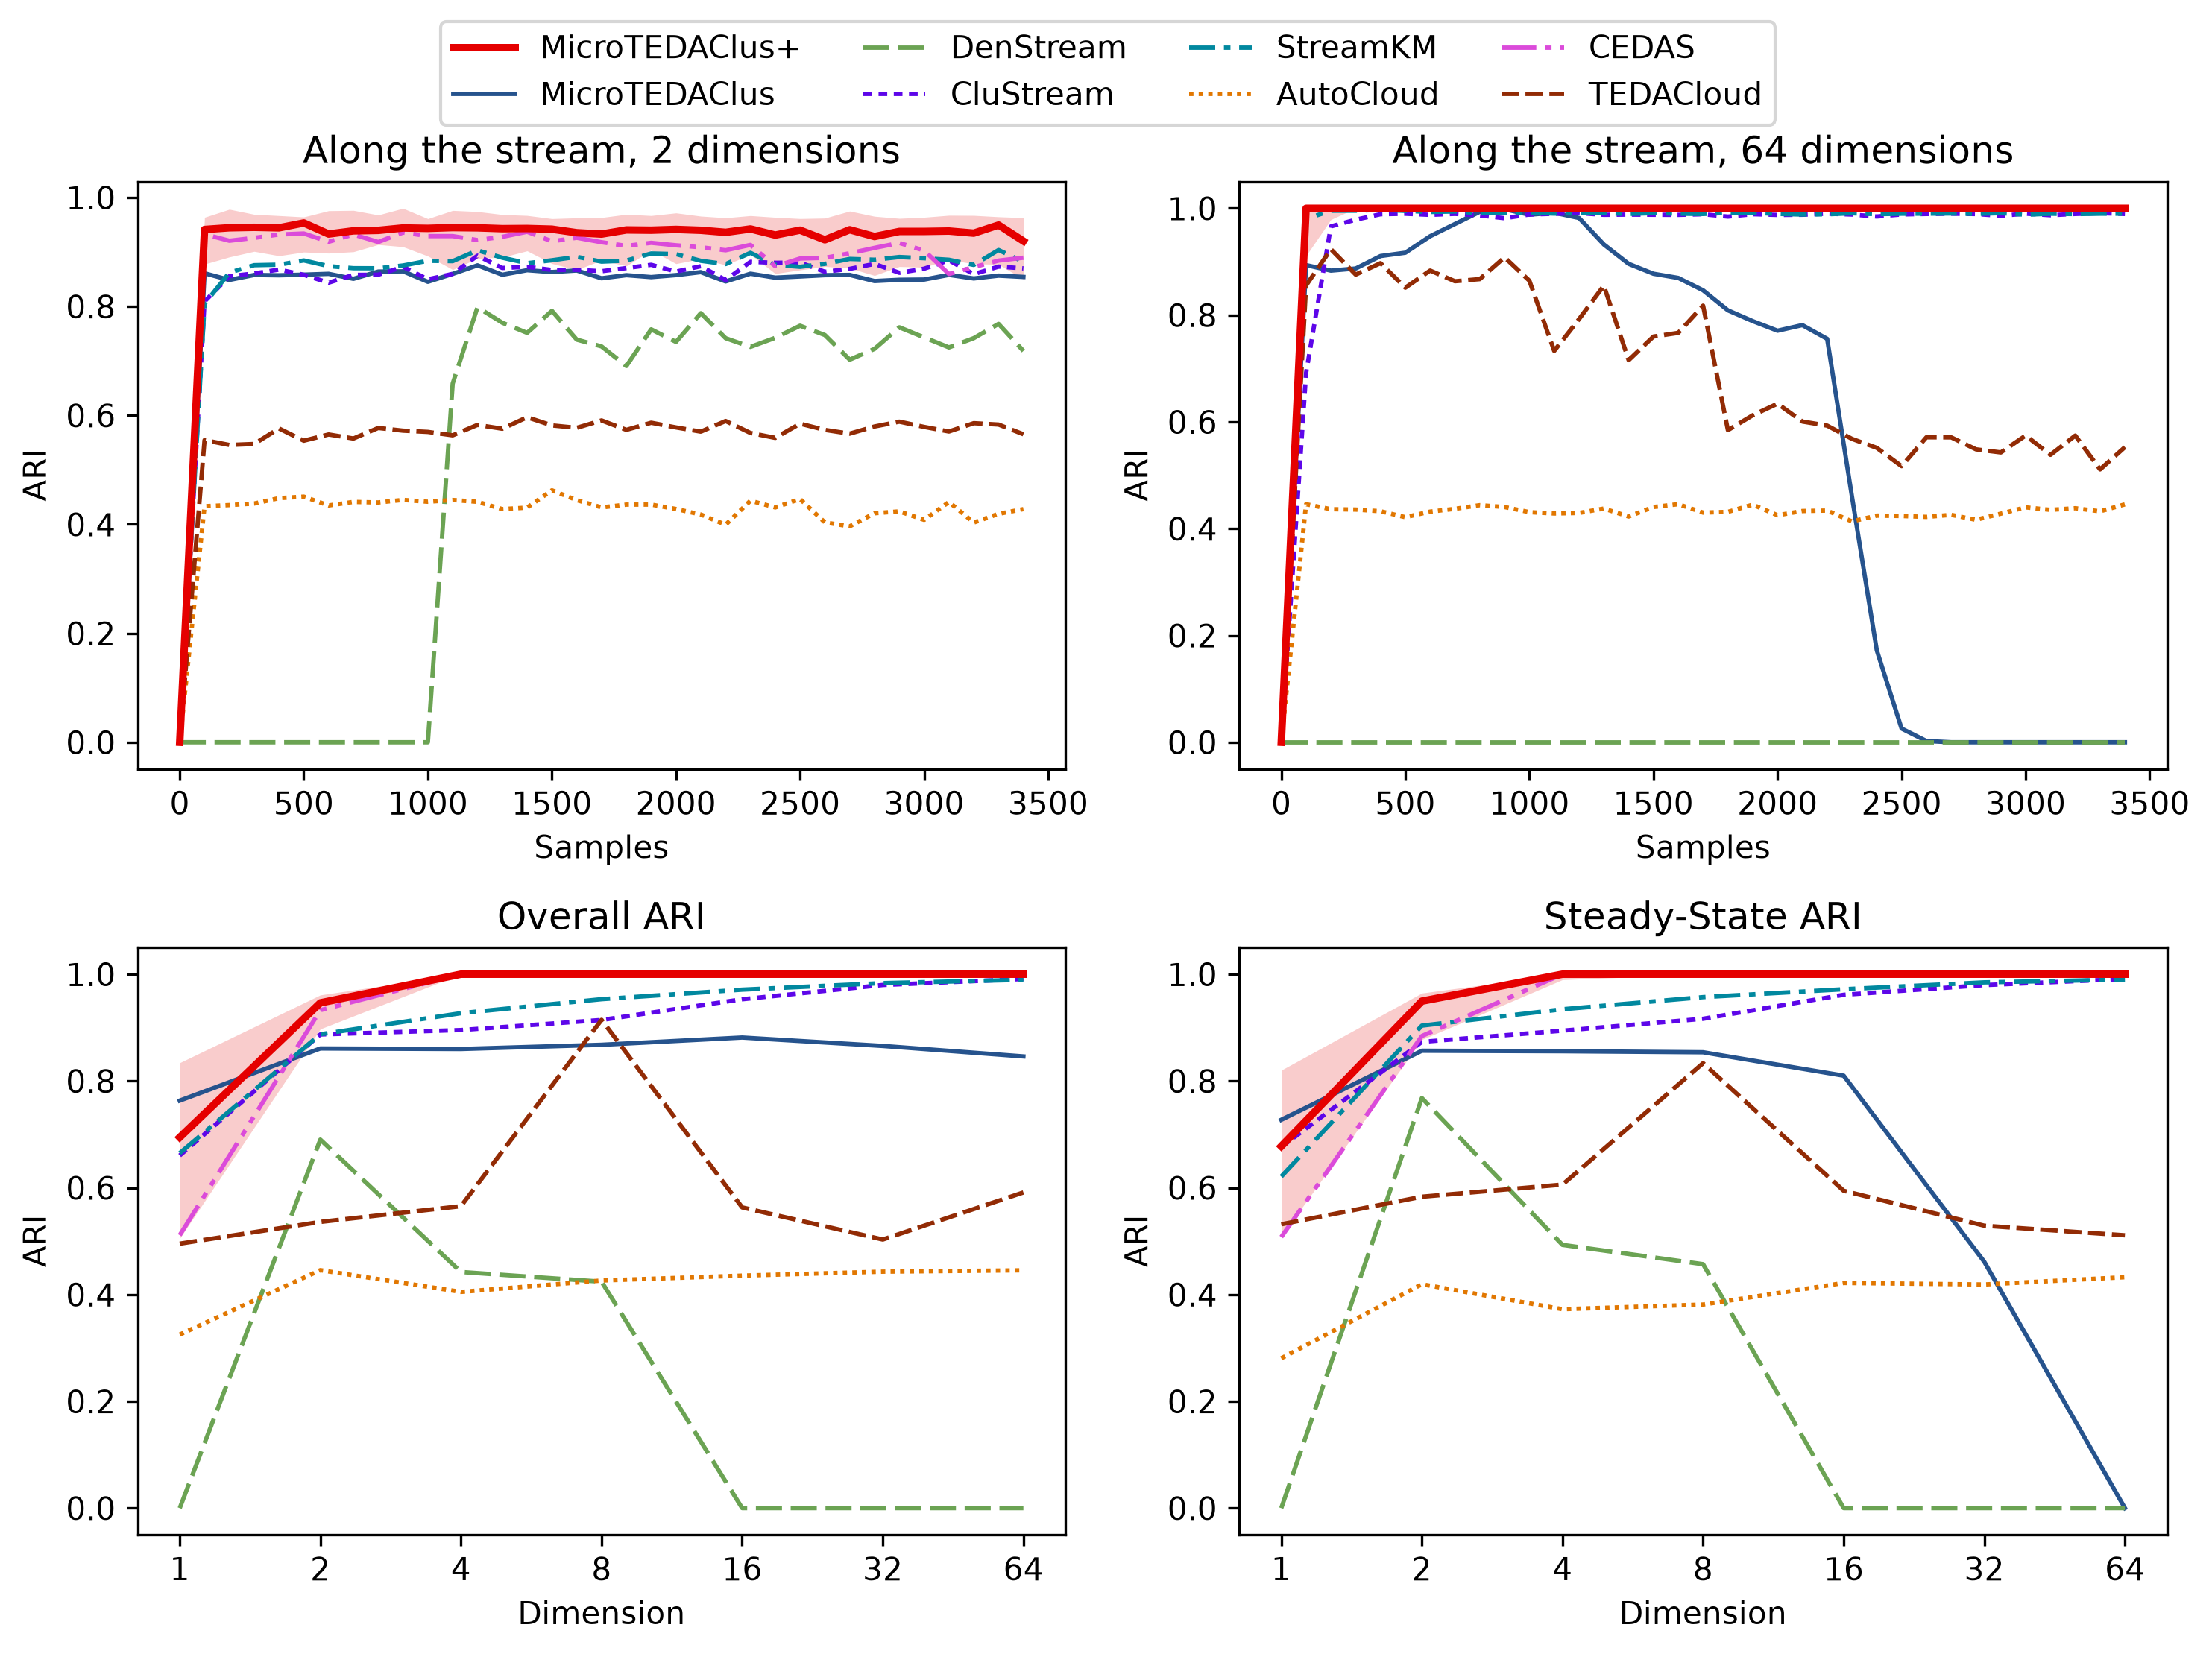
\includegraphics[height=0.8\textheight]{ModelImprovement/artifacts/comparison/plots/scalability_quality.png}
  \note{- Red: MicroTEDAClus+, better than every model but CEDAS from two dimensions on}
\end{frame}

% -----------------------------------------------------------------------------
\section{Conclusions}

\begin{frame}{Conclusions}
  \begin{itemize}
    \item The formulation has issues of its own, and the implementation behind the results departs from it
    \item The original methodology leaks information and evaluates each batch after learning it
    \item Under a methodology without these flaws, \MicroTEDAClus is not on par with the benchmark models, nor better under concept drift
    \item \MicroTEDAClusPlus improves on it in quality, time and memory, and no benchmark model is better under concept drift
  \end{itemize}
  \note{- The objectives a to d are met}
\end{frame}

\begin{frame}{Contributions}
  \begin{itemize}
    \item The reassessment of the formulation, the implementation and the methodology
    \item The methodology that replaces it
    \item The vectorized implementation
    \item The experiments of the improvement
    \item \MicroTEDAClusPlus
    \item Code and sources, public~\cite{carvalho2026microtedaclusreassessment}
  \end{itemize}
  \note{- The repository: last slide}
\end{frame}

\begin{frame}{Limits and future work}
  \begin{columns}[t]
    \column{0.48\textwidth}
    \textbf{Limits}
    \begin{itemize}
      \item Streams that repeat: the Chameleon datasets are fixed files
      \item The search as a source of variation
      \item Cost measures implementations
      \item Synthetic data of up to 64 dimensions
    \end{itemize}
    \column{0.48\textwidth}
    \textbf{Future work}
    \begin{itemize}
      \item Hyperparameter selection
      \item The static shapes
      \item Searching whether to label noise
      \item Fast prediction as a strength
    \end{itemize}
  \end{columns}
  \note{- Each limit bounds a claim, not the method}
\end{frame}

\begin{frame}{Thank you}
  \centering
  \vfill
  {\Large Thank you for your presence}\\[1.5em]
  \qrcode[height=3cm]{https://github.com/eduardo-ufmg/microtedaclus-reassessment/tree/thesis-defense}\\[0.8em]
  \footnotesize\url{https://github.com/eduardo-ufmg/microtedaclus-reassessment}
  \vfill
  \note{- Open to the questions of the board}
\end{frame}

\begin{frame}[allowframebreaks]{References}
  \footnotesize
  \bibliographystyle{abntex2-num}
  \bibliography{../monografia/References}
\end{frame}

% -----------------------------------------------------------------------------
\appendix
\section{Appendix}

\begin{frame}{Corrections}
  \placeholder{\textwidth}{0.75\textheight}{Correction candidates and their results\\(from the tables of Section 4.3)}
\end{frame}

\begin{frame}{Improvements}
  \placeholder{\textwidth}{0.75\textheight}{Improvement candidates and their results\\(from the tables of Section 4.4)}
\end{frame}

\begin{frame}{Statistical tests}
  \placeholder{\textwidth}{0.75\textheight}{Paired Wilcoxon, Holm across datasets, Cliff's delta\\(from Section 3.7)}
\end{frame}

\begin{frame}{The number of runs}
  \placeholder{\textwidth}{0.75\textheight}{Kneedle on the worst-case convergence curve of the median\\(from Section 3.6.2)}
\end{frame}

\begin{frame}{The interface measurement}
  \centering
  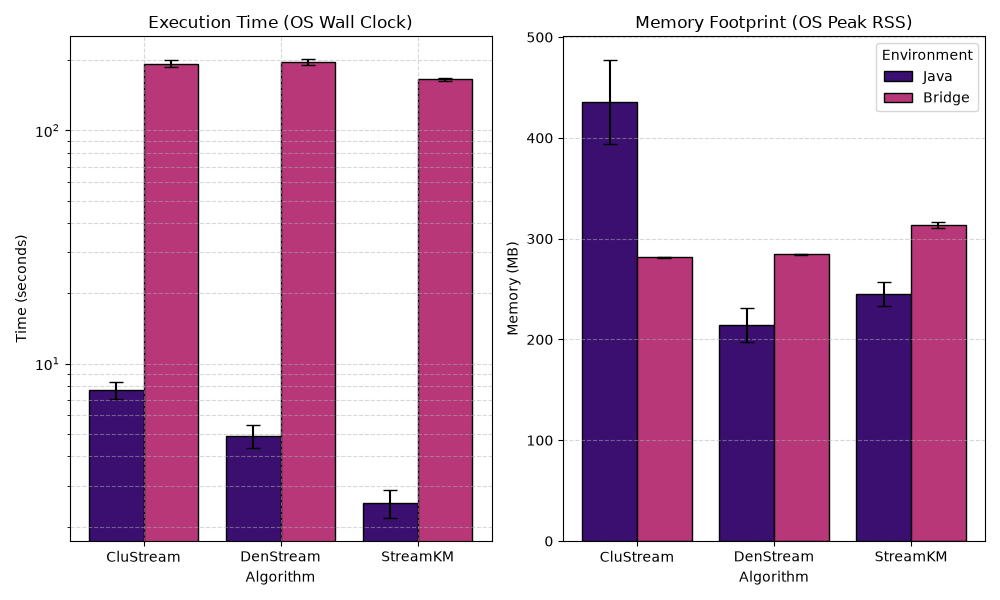
\includegraphics[height=0.75\textheight]{MethodologyReassessment/figures/benchmark_java_bridge.png}
\end{frame}

\begin{frame}{Other departures of the implementation}
  \placeholder{\textwidth}{0.75\textheight}{Two-pass macroclusters, the factor $4/d^2$, the membership\\(from Section 3.1)}
\end{frame}

\begin{frame}{The selection probe}
  \placeholder{\textwidth}{0.75\textheight}{The search space holds better configurations than those selected\\(from Section 4.6)}
\end{frame}

\begin{frame}{Hyperparameters}
  \placeholder{\textwidth}{0.75\textheight}{The variance limit of \MicroTEDAClus and the relative limit of \MicroTEDAClusPlus\\(from Sections 3.8 and 4.8)}
\end{frame}

\begin{frame}{Datasets}
  \placeholder{\textwidth}{0.75\textheight}{Concept drift streams, static shapes, scalability streams\\(from Section 3.3)}
\end{frame}

\end{document}
